\documentclass[main.tex]{subfiles}
\begin{document}

\section{Neural Compositional Denotational Semantics for Question Answering} % 3pp
\label{sec:denotation-semantics}

\subsection{Introduction}
In our model in chapter 2 and 3 the parser uses Seq2Seq (w/ attention) encoder-decoder architecture to encode the question as a dense vector and then decode a program (in a grammar-constrained manner) using this vector with attention to input tokens.  Since the program-decoding is not tied to the input utterance explicitly, as opposed to parsers used before~\cite{zettlemoyer-pccg-2005,instructaction-artzi-2013,pasupat-liang-2015}, such an architecture does not guarantee generalization to novel combinations of sub-utterances.
Additionally, our model's symbolic reasoning capability is limited to operations that are pre-defined in the module-set of the model.  This does not allow for automatic discovery of new discrete operations based on question-denotation supervision.  In this chapter we present a model that pushes in both these directions.


% Compositionality is a mechanism by which the meanings of complex expressions are systematically determined from the meanings of their parts, and has been widely assumed in the study of both artificial and natural languages~\cite{montague-semantics} as a means for allowing speakers to generalize to understanding an infinite number of sentences. Popular neural network approaches to question answering use a restricted form of compositionality, typically encoding a sentence word-by-word, and then executing the complete sentence encoding against a knowledge source. Such models can fail to generalize from training data in surprising ways.
Inspired by linguistic theories of compositional semantics, we propose a parser that builds a latent tree of interpretable expressions over a sentence, recursively combining constituents using a small set of neural modules. % Our model outperforms RNN encoders, particularly when test questions are longer than training questions.
Our approach resembles Montague semantics~\cite{montague-semantics}, in which a tree of interpretable expressions is built over the sentence, with nodes combined by a small set of composition functions. %The interpretation of the complete sentence corresponds to the answer to a question.
However, both the structure of the sentence and the composition functions are learned by end-to-end gradient descent. To achieve this, we define the parametric form of small set of composition modules, and then build a parse chart over each sentence subsuming all possible trees. Each node in the chart represents a span of text with a distribution over groundings (in terms of booleans and knowledge base nodes and edges), as well as a vector representing aspects of the meaning that have not yet been grounded. The representation for a node is built by taking a weighted sum over different ways of building the node. % The trees induced by our model are linguistically plausible, in contrast to prior work on structure learning from semantic objectives~\cite{williams-latenttree-2018}.

% Typical neural approaches to grounded question answering first encode a question with a recurrent neural network (RNN), and then evaluate the encoding against an encoding of the knowledge source (for example, a knowledge graph or image) \citep{SantoroRBMPBL17}.
% In contrast to classical approaches to compositionality, constituents of complex expressions are not given explicit interpretations in isolation.
% For example, in \emph{Which cubes are large or green?}, an RNN encoder will not explicitly build an interpretation for the phrase \emph{large or green}.
% We show that such approaches can generalize poorly when tested on more complex sentences than they were trained on.
%Such approaches have been shown weak generalization performance in some respects.
Our approach imposes independence assumptions that give a linguistically motivated inductive bias. In particular, it enforces that phrases are interpreted independently of surrounding words, allowing the model to generalize naturally to interpreting phrases in different contexts. In our model, \emph{large or green} will be represented as a particular set of entities in a knowledge graph, and be intersected with the set of entities represented by the \emph{cubes} node.  We show that this inductive bias allows our model to generalize well when tested on more complex sentences than it was trained on.  We also show that our model learns a variety of challenging semantic operators, such as quantifiers, disjunctions and composed relations, without being explictly defined to do so.

%Another perspective on our work is as a method for learning the layouts of Neural Module Networks (NMNs) \citep{andreas2016neural}.
% Another perspective on our work is as a method for learning layouts of Neural Module Networks (NMNs)~\cite{nmn-2016}.
% Work on NMNs has focused on construction of the structure of the network, variously using rules, parsers and reinforcement learning \citep{Andreas2016LearningTC, Hu2017LearningTR}. Our end-to-end differentiable model jointly learns structures and modules by gradient descent.

% Our model is a new combination of classical and neural methods, which maintains the interpretability and generalization behaviour of semantic parsing, while being end-to-end differentiable.

\begin{figure}[tb]
    \centering
    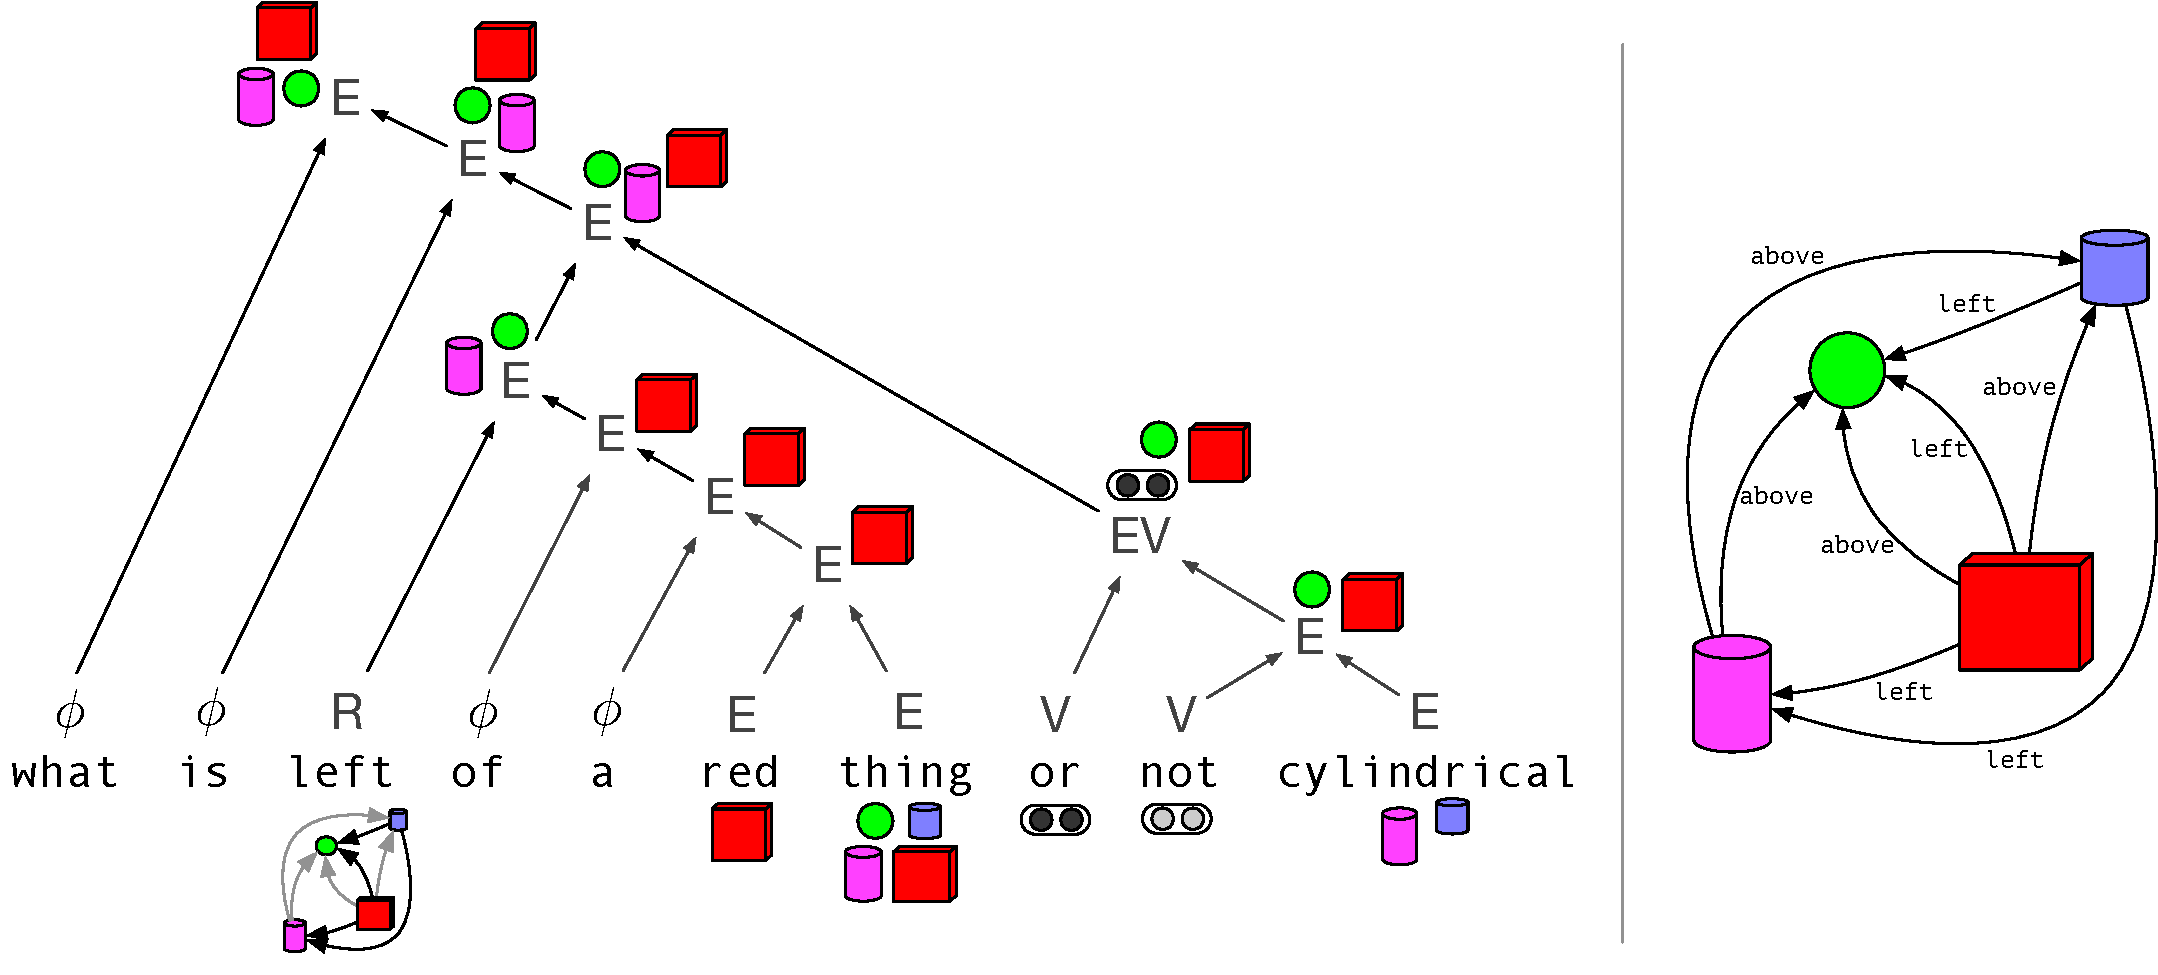
\includegraphics[width=\textwidth]{chapter-4/04-overview.pdf}
    \caption{{ A correct parse for a question given the knowledge graph on the right, using our model. We show the type for each node, and its denotation in terms of the knowledge graph. The words \emph{or} and \emph{not} are represented by vectors, which parameterize composition modules. The denotation for the complete question represents the answer to the question.
    Nodes here have types $E$ for sets of entities, $R$ for relations, $V$ for ungrounded vectors, $EV$ for a combination of entities and a vector, and $\phi$ for semantically vacuous nodes.
    While we show only one parse tree here, our model builds a parse chart subsuming all trees.} }
    \label{fig:04-overview}
\end{figure}



\subsection{Model Overview}
\label{sec:model}
Our task is to answer a question $q=w_{1..|q|}$, with respect to a Knowledge Graph (KG) consisting of nodes $\E$ (representing entities) and labelled directed edges $\R$ (representing relationship between entities). In our task, answers are either booleans, or specific subsets of nodes from the KG.

Our model builds a parse for the sentence, in which phrases are grounded in the KG, and a small set of composition modules are used to combine phrases, resulting in a grounding for the complete question sentence that answers it. For example, in Figure~\ref{fig:04-overview}, the phrases \emph{not} and \emph{cylindrical} are interpreted as a function word and an entity set, respectively, and then \emph{not cylindrical} is interpreted by computing the complement of the entity set.

The node at the root of the parse tree is the answer to the question.
Our model answers questions by:

\paragraph{(a)} Grounding individual tokens in a KG, that can either be grounded as particular sets of entities and relations in the KG, as ungrounded vectors, or marked as being semantically vacuous. For each word, we learn parameters that are used to compute a distribution over semantic types and corresponding denotations in a KG (\S~\ref{sssec:semtype}).

\paragraph{(b)} Combining representations for adjacent phrases into representations for larger phrases, using trainable neural composition modules (\S~\ref{sssec:comprules}). This produces a denotation for the phrase.

\paragraph{(c)} Assigning a binary-tree structure to the question sentence, which determines how words are grounded, and which phrases are combined using which modules. We build a parse chart subsuming all possible structures, and train a parsing model to increase the likelihood of structures leading to the correct answer to questions. Different parses leading to a denotation for a phrase of type $t$ are merged into an expected denotation, allowing dynamic programming (\S~\ref{ssec:parsing}).

\paragraph{(d)} Answering the question, with the most likely grounding of the phrase spanning the sentence.


\subsection{Compositional Semantics}
\subsubsection{Semantic Types}
\label{sssec:semtype}
Our model classifies spans of text into different semantic types to represent their meaning as explicit denotations, or ungrounded vectors.
All phrases are assigned a distribution over semantic types.
The semantic type determines how a phrase is grounded, and which composition modules can be used to combine it with other phrases.
A phrase spanning $w_{i..j}$ has a denotation $\llbracket w_{i..j} \rrbracket_{KG}^{t}$ for each semantic type $t$.
For example, in Figure \ref{fig:04-overview}, \emph{red} corresponds to a set of entities, \emph{left} corresponds to a set of relations, and \emph{not} is treated as an ungrounded vector. %Each phrase has a representation for all types, with some probability.

The semantic types we define can be classified into three broad categories. \textit{We omit details for brevity and refer the reader to the paper~\cite{gupta-ncds-2018} for details.}

\paragraph{Grounded Semantic Types:} Spans of text that can be fully grounded in the KG. %For example, in Figure \ref{}, phrases such as

\begin{enumerate}
    \item
    {\bf Entity} (\semtype{E}): Spans of text that can be grounded to a set of entities in the KG, for example, \emph{red sphere} or \emph{large cube}.
    % \semtype{E}-type span grounding is represented as an attention value for each entity, $[p_{e_{1}}, \ldots, p_{e_{|\E|}}]$, where $p_{e_{i}} \in [0, 1]$. % $0 \leq p_{e_{i}} \leq 1$.
    % This can be viewed as a soft version of a logical set-valued denotation, which we refer to as a soft entity set.

    \item
    {\bf Relation} (\semtype{R}): Spans of text that can be grounded to set of relations in the KG, for example, \emph{left of} or \emph{not right of or above}. % can be grounded as subsets of KG edges.
    \semtype{R}-type span grounding is represented by a soft adjacency matrix. % $A \in \mathbb{R}^{|\E|\times|\E|}$ where $A_{ij} = 1$ denotes a directed edge from $e_{i} \rightarrow e_{j}$.

    \item
    {\bf Truth} (\semtype{T}): Spans of text that can be grounded with a Boolean denotation, for example, \emph{Is anything red?}, \emph{Is one ball green and are no cubes red?}.
    % \semtype{T}-type span grounding is represented using a real-value $p_{true} \in [0,1]$ that denotes the probability of the span being true.
\end{enumerate}

\paragraph{Ungrounded Semantic Types:} Spans of text whose meaning cannot be grounded in the KG.

\begin{enumerate}%[nolistsep, noitemsep]
% \noindent
\item
{\bf Vector} (\semtype{V}):
    This type is used for spans representing functions that cannot yet be grounded in the KG (e.g. words such as \emph{and} or \emph{every}).
    These spans are represented using $4$ different real-valued vectors $v_{1}$-$v_{4}$ $\in$ $\mathbb{R}^{2}$-$\mathbb{R}^{5}$, that are used to parameterize the composition modules described in \S \ref{sssec:comprules}.


    \item
    {\bf Vacuous} ($\pmb{\phi}$): Spans that are considered semantically vacuous, but are necessary syntactically, e.g. \emph{of} in \emph{left of a cube}. During composition, these nodes act as identity functions. %Language spans that do not contribute any meaning to the interpretation of the question or removing which will not change the meaning of the question (in most cases) belong to this semantic type. \todo{text that appears for grammatical consistency and completeness} For example, ``that is'',
\end{enumerate}


\begin{figure}[h!]
  \captionsetup[subfigure]{labelformat=empty}
  \begin{subfigure}[t]{.48\textwidth}
    \centering
    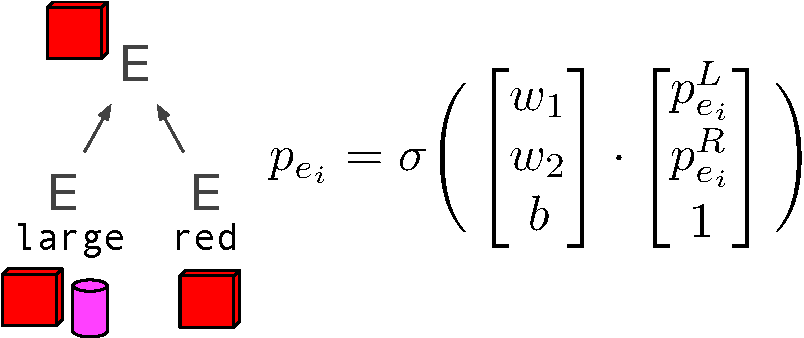
\includegraphics[width=0.5\linewidth]{chapter-4/E+E=E_new.pdf}
    \caption{\label{fig:eee} \scriptsize{\semtype{E} + \semtype{E} $\rightarrow$ \semtype{E}: This module performs a function on a pair of soft entity sets, parameterized by the model's global parameter vector $[w_{1}, w_{2}, b]$ to produce a new soft entity set. The composition function for a single entity's resulting attention value is shown. Such a composition module can be used to interpret compound nouns and entity appositions. For example, the composition module shown above learns to output the intersection of two entity sets.}}
  \end{subfigure}
  \hfill
  \begin{subfigure}[t]{.48\textwidth}
    \centering
    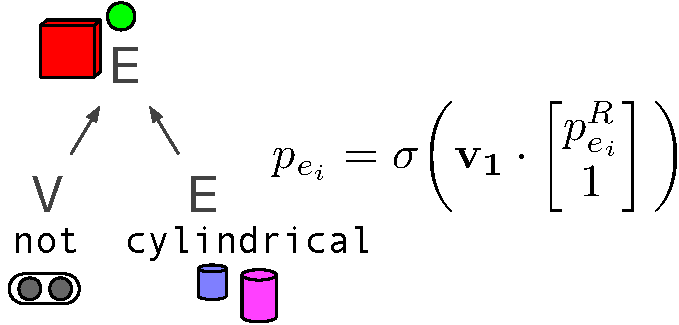
\includegraphics[width=0.5\linewidth]{chapter-4/W+E=E_new.pdf}
    \caption{\label{fig:wee}\scriptsize{\semtype{V} + \semtype{E} $\rightarrow$ \semtype{E}: This module performs a function on a soft entity set, parameterized by a word vector, to produce a new soft entity set. For example, the word \emph{not} learns to take the complement of a set of entities. The entity attention representation of the resulting span is computed by using the indicated function that takes the $v_{1} \in \mathbb{R}^{2}$ vector of the \semtype{V} constituent as a          parameter argument and the entity attention vector of the \semtype{E} constituent as a function argument.}}
  \end{subfigure}

    \smallskip

  \begin{subfigure}[t]{.48\textwidth}
    \centering
    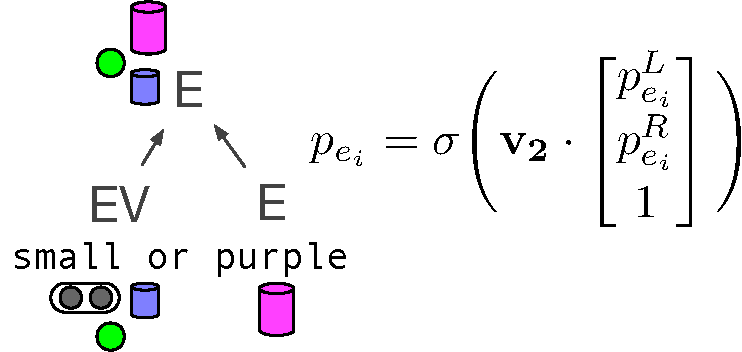
\includegraphics[width=0.6\linewidth]{chapter-4/EW+E=E_new.pdf}
    \caption{\label{fig:ewee} \scriptsize{\semtype{EV} + \semtype{E} $\rightarrow$ \semtype{E}: This module combines two soft entity sets into a third set, parameterized by the $v_{2}$ word vector. This composition function is similar to a linear threshold unit and is capable of modeling various mathematical operations such as logical conjunctions, disjunctions, differences etc. for different values of $v_{2}$. For example, the word \emph{or} learns to model set union.}}
  \end{subfigure}
  \hfill
  \begin{subfigure}[t]{.48\textwidth}
    \centering
    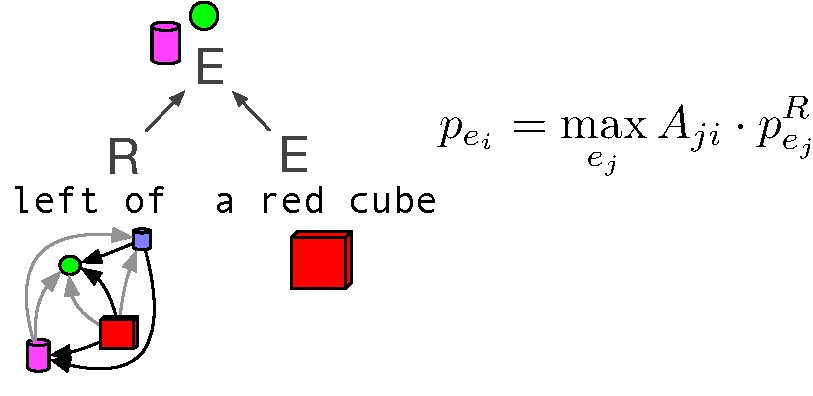
\includegraphics[width=0.6\linewidth]{chapter-4/R+E=E_new.pdf}
    \caption{\label{fig:ree}\scriptsize{\semtype{R} + \semtype{E} $\rightarrow$ \semtype{E}: This module composes a set of relations (represented as a single soft adjacency matrix) and a soft entity set to produce an output soft entity set. The composition function uses the adjacency matrix representation of the \semtype{R}-span and the soft entity set representation of the \semtype{E}-span. }}
  \end{subfigure}

   \smallskip
    % \medskip

  \begin{subfigure}[t]{.48\textwidth}
    \centering
    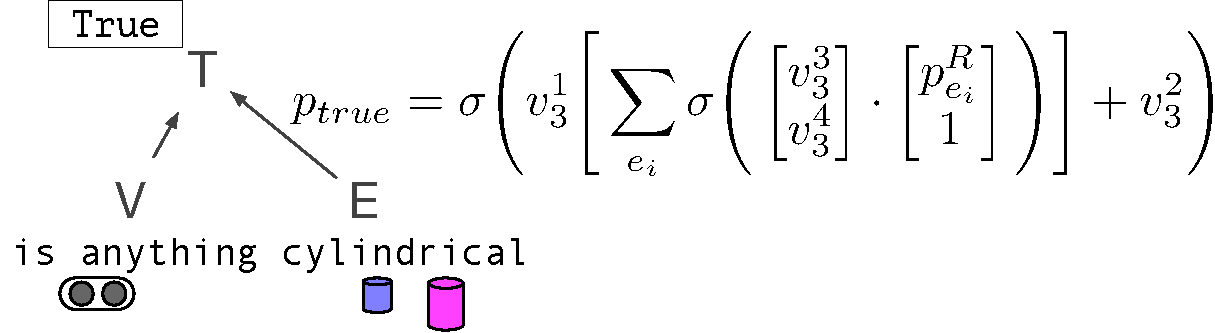
\includegraphics[width=0.85\linewidth]{chapter-4/W+E=B_new.pdf}
    \caption{\label{fig:web}\scriptsize{\semtype{V} + \semtype{E} $\rightarrow$ \semtype{T}: This module maps a soft entity set onto a soft boolean, parameterized by word vector ($v_{3}$).  The module counts whether a sufficient number of elements are in (or out) of the set. For example, the word \emph{any} should test if a set is non-empty.}}
  \end{subfigure}
  \hfill
  \begin{subfigure}[t]{.48\textwidth}
    \centering
    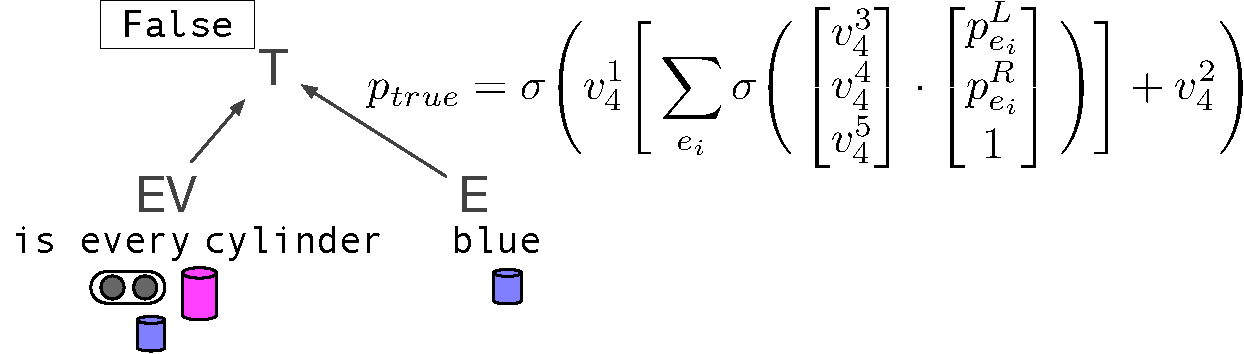
\includegraphics[width=0.85\linewidth]{chapter-4/EW+E=B_new.pdf}
    \caption{\label{fig:eweb}\scriptsize{\semtype{EV} + \semtype{E} $\rightarrow$ \semtype{T}: This module combines two soft entity sets into a soft boolean, which is useful for     modelling generalized quantifiers. For example, in \emph{is every cylinder blue}, the module can use the inner sigmoid to test if an element $e_i$ is in the set of cylinders ($p^{L}_{e_{i}}\approx 1$) but not in the set of blue things ($p^{R}_{e_{i}}\approx 0$), and then use the outer sigmoid to return a value close to 1 if the sum of elements matching this property is close to 0.  }}
  \end{subfigure}

   \smallskip
   % \medskip

  \begin{subfigure}[t]{.48\textwidth}
    \centering
    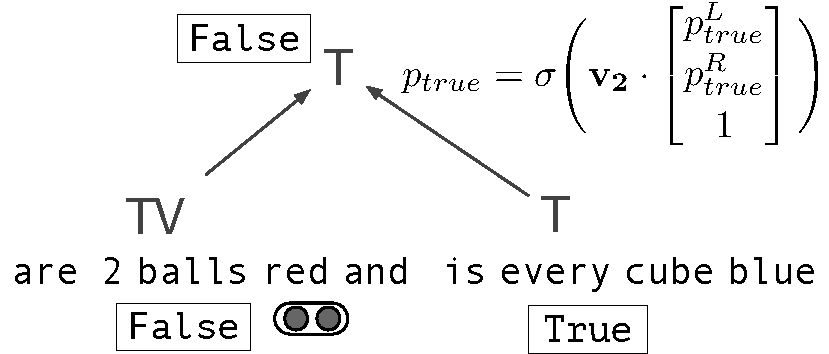
\includegraphics[width=0.6\linewidth]{chapter-4/BW+B=B_new.pdf}
    \caption{\label{fig:bwbb}\scriptsize{\semtype{TV} + \semtype{T} $\rightarrow$ \semtype{T}: This module maps a pair of soft booleans into a soft boolean using the $v_{2}$ word vector to parameterize the composition function. Similar to \semtype{EV}~+~\semtype{E}~$\rightarrow$~\semtype{E}, this module facilitates modeling a range of boolean set operations. Using the same functional form for different composition functions allows our model to use the same ungrounded word vector ($v_{2}$) for compositions that are semantically analogous.}}
  \end{subfigure}
  \hfill
  \begin{subfigure}[t]{.48\textwidth}
    \centering
    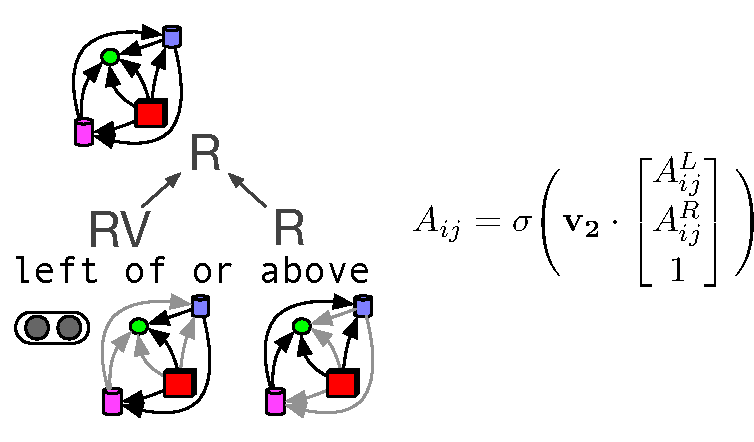
\includegraphics[width=0.6\linewidth]{chapter-4/RW+R=R_new.pdf}
    \caption{\label{fig:rwrr}\scriptsize{\semtype{RV} + \semtype{R} $\rightarrow$ \semtype{R}: This module composes a pair of soft set of relations to a produce an output soft set of relations. For example, the relations \emph{left} and \emph{above} are composed by the word \emph{or} to produce a set of relations such that entities $e_{i}$ and $e_{j}$ are related if either of the two relations exists between them. The functional form for this composition is similar to \semtype{EV}~+~\semtype{E}~$\rightarrow$~\semtype{E} and \semtype{TV}~+~\semtype{T}~$\rightarrow$~\semtype{T} modules. }}
  \end{subfigure}

  \caption{\label{fig:04-modules} \footnotesize{Composition Modules that compose two constituent span representations into the representation for the combined larger span, using the indicated equations.}}
\end{figure}


\paragraph{Partially-Grounded Semantic Types:}
Spans of text that can only be partially grounded in the knowledge graph, such as \emph{and red} or \emph{are four spheres}. Here, we represent the span by a combination of a grounding and vectors, representing grounded and ungrounded aspects of meaning respectively.
The grounded component of the representation will typically combine with another fully grounded representation, and the ungrounded vectors will parameterize the composition module.
We define 3 semantic types of this kind: \semtype{EV}, \semtype{RV} and \semtype{TV}, corresponding to the combination of entities, relations and boolean groundings respectively with an ungrounded vector. Here, the word represented by the vectors can be viewed as a binary function, one of whose arguments has been supplied.


\subsubsection{Composition Modules}
\label{sssec:comprules}
Next, we describe how we compose phrase representations (from \S~\ref{sssec:semtype}) to represent larger phrases.
We define a small set of composition modules, that take as input two constituents of text with their corresponding semantic representations (grounded representations and ungrounded vectors), and outputs the semantic type and corresponding representation of the larger constituent.
The composition modules are parameterized by the trainable word vectors.
These can be divided into several categories:

\paragraph{Composition modules resulting in fully grounded denotations:} Described in Figure~\ref{fig:04-modules}.
\textit{For some reason, this figure appears at the end of the proposal document; I will fix it.}



\paragraph{Composition with $\pmb{\phi}$-typed nodes:} Phrases with type $\pmb{\phi}$ are treated as being semantically transparent identity functions. Phrases of any other type can combined with these nodes, with no change to their type or representation.

\paragraph{Composition modules resulting in partially grounded denotations:} We define several modules that combine fully grounded phrases with ungrounded phrases, by deterministically taking the union of the representations, giving phrases with partially grounded representations (\S~\ref{sssec:semtype}). These modules are useful when words act as binary functions; here they combine with their first argument. For example, in Fig.~\ref{fig:04-overview}, \emph{or} and \emph{not cylindrical} combine to make a phrase containing both the vectors for \emph{or} and the entity set for \emph{not cylindrical}.


\subsection{Parsing Model}
\label{ssec:parsing}
Here, we describe how our model classifies question tokens into semantic type spans and computes their representations (\S~\ref{sssec:leaf}), and recursively uses the composition modules defined above to parse the question into a soft latent tree that provides the answer (\S~\ref{sssec:parse}). The model is trained end-to-end using only question-answer supervision.


\subsubsection{Lexical Representation Assignment}
\label{sssec:leaf}
Each token in the question sentence is assigned a distribution over the semantic types, and a grounded representation for each type. Tokens can only be assigned the \semtype{E}, \semtype{R}, \semtype{V}, and $\pmb{\phi}$ types.
For example, the token \emph{cylindrical} in the question in Fig.~\ref{fig:04-overview} is assigned a distribution over the $4$ semantic types (one shown) and for the \semtype{E} type, its representation is the set of \textit{cylindrical} entities.

\paragraph{Semantic Type Distribution for Tokens:} To compute the semantic type distribution, our model represents each word $w$, and each semantic type $t$ using an embedding vector; $v_{w}, v_{t} \in \mathbb{R}^{d}$. The semantic type distribution is assigned with a softmax:
\begin{equation*}
    p(t|w_{i}) \propto \exp({v_{t}\cdot v_{w_{i}}})
    \label{eq:wordtypdist}
\end{equation*}

\paragraph{Grounding for Tokens:}
For each of the semantic type, we assign their denotation in a fairly simple manner.
\semtype{E}-Type representation is assigned by locally normalizing the dot-product score between a token's word embedding and the entity vector, for each entity in the KG.
\semtype{R}-Type representation is an expected adjecency matrix computed under the token-relation affinity distribution. This distribution is obtained by normalizing the dot-product score between the token's and relation's embedding.
\semtype{V}-Type representation are four additional word vectors that are learned for each word in the vocabulary.
$\pmb{\phi}$-type is vacuous and does not require a representation.
Please refer to the accompanying paper~\cite{gupta-ncds-2018} for details.


\subsubsection{Parsing Questions}
\label{sssec:parse}
To learn the correct structure for applying composition modules, we use a simple parsing model. We build a parse-chart over the question encompassing all possible trees by applying all composition modules, similar to a standard CRF-based PCFG parser using the CKY algorithm.
Each node in the parse-chart, for each span $w_{i..j}$ of the question, is represented as a distribution over different semantic types with their corresponding representations. %This distribution is computed by weighing the different ways of composing the span's constituents.
We omit details for brevity; please refer to the accompanying paper~\cite{gupta-ncds-2018} for details.


\paragraph{Answer Grounding:}
By recursively computing the phrase semantic-type potentials and representations, we can infer the semantic type distribution of the complete question and the resulting grounding for different semantic types $t$, $\llbracket w_{1..|q|} \rrbracket_{KG}^{t}$.
\begin{equation}
\label{eq:qtd}
    p(t|q) \propto \psi(1, |q|, t)
\end{equation}
The answer-type (boolean or subset of entities) for the question is computed using:
\begin{equation}
    t^{*} = \argmax_{t \in {\semtype{T}, \semtype{E}}} \; p(t|q)
\end{equation}
The corresponding grounding is $\llbracket w_{1..|q|} \rrbracket_{KG}^{t^{*}}$, which answers the question.


% \subsection{Training Objective}
% \label{sssec:train}

\subsection{Experiments}
\label{ssec:exp}

\paragraph{Dataset}
We generate a dataset of question and answers based on the \textsc{CLEVR} dataset~\cite{clevr-2017}, which contains knowledge graphs containing attribute information of objects and relations between them.

We generate a new set of questions as existing questions contain some biases that can be exploited by models.\footnote{
\newcite{clevr-2017} found that many spatial relation questions can be answered only using absolute spatial information, and many long questions can be answered correctly without performing all steps of reasoning. We employ some simple tests to remove trivial biases from our dataset.}
We generate 75K questions for training and 37.5K for validation.
Our questions test various challenging semantic operators.
These include conjunctions (e.g. \emph{Is anything red and large?}), negations (e.g. \emph{What is not spherical?}), counts (e.g. \emph{Are five spheres green?}), quantifiers (e.g. \emph{Is every red thing cylindrical?}), and relations (e.g. \emph{What is left of and above a cube?}). We create two test sets:

\begin{enumerate}
\item
\textbf{Short Questions:}
Drawn from the same distribution as the training data (37.5K).

\item
\textbf{Complex Questions:}
Longer questions than the training data (22.5K). This test set contains the same words and constructions, but chained into longer questions.
For example, it contains questions such as \emph{What is a cube that is right of a metallic thing that is beneath a blue sphere?} and \emph{Are two red cylinders that are above a sphere metallic?}
Solving these questions require more multi-step reasoning.
\end{enumerate}

% Our experiments investigate the ability of our model to understand complex synthetic and natural language queries, learn interpretable structure, and generalize compositionally.
% We also isolate the effect of learning the syntactic structure and representing sub-phrases using explicit denotations.

We also experiment with Referring Expression Generation (GenX) dataset~\cite{refexp-fitzgerald-2013} and refer the reader to our paper to read about experiments related to it.



\paragraph{Baseline Models:}
We compare to the following baselines.
\textbf{(a)} Models that assume linear structure of language, and encode the question using linear RNNs---\textsc{LSTM (No KG)}, \textsc{LSTM}, \textsc{Bi-LSTM}, and a \textsc{Relation-Network}~\cite{relnet-santoro-2017} augmented model.
% \footnote{We use this baseline only for {\sc CLEVRGEN} since {\sc GenX} does not contain relations.}
\textbf{(b)} Models that assume tree-like structure of language. We compare two variants of Tree-structured LSTMs~\cite{recursivelstm-zhu-2015,treelstm-tai-2015}---\textsc{Tree-LSTM}, that operates on pre-parsed questions, and \textsc{Tree-LSTM(Unsup.)}, an unsupervised Tree-LSTM model~\cite{malliard-unsuptree-2017} that learns to jointly parse and represent the sentence.
% For {\sc GenX}, we also use an end-to-end semantic parsing model from \citet{Pasupat2015CompositionalSP}.
Finally, to isolate the contribution of the proposed denotational-semantics model, we train our model on pre-parsed questions.
Note that, all LSTM based models only have access to the entities of the KG but not the relationship information between them.


\paragraph{Short Questions Performance:}
Table~\ref{tab:04-qa} shows that our model perfectly answers all test questions, demonstrating that it can learn challenging semantic operators and induce parse trees from end task supervision.

\paragraph{Complex Questions Performance:}
Table~\ref{tab:04-longerqa} shows results on complex questions, which are constructed by combining components of shorter questions.
These require complex multi-hop reasoning, and the ability to generalize robustly to new types of questions.
We use the same models as in Table~\ref{tab:04-qa}, which were trained on short questions.
All baselines achieve close to random performance, despite high accuracy for shorter questions. This shows the challenges in generalizing RNN encoders
beyond their training data.
In contrast, the strong inductive bias from our model structure allows it to generalize well to  complex questions.
Our model outperforms \textsc{Tree-LSTM (Unsup.)} and the version of our model that uses pre-parsed questions, showing the effectiveness of explicit denotations and learning the syntax, respectively.

\begin{table}[tb]
\centering
\footnotesize
\begin{tabular}{l c c c c}
\toprule
\bf Model & \bf Boolean Questions & \bf Entity Set Questions & \bf Relation Questions & \bf Overall \\
\midrule
\textsc{LSTM (No KG)}               & 50.7 & 14.4 & 17.5  & 27.2 \\
\textsc{LSTM }                      & 88.5 & 99.9 & 15.7  & 84.9 \\
\textsc{Bi-LSTM }                   & 85.3 & 99.6 & 14.9  & 83.6 \\
\textsc{Tree-LSTM}                  & 82.2 & 97.0 & 15.7  & 81.2 \\
\textsc{Tree-LSTM (Unsup.)}         & 85.4 & 99.4 & 16.1  & 83.6 \\
\textsc{Relation Network}           & 85.6 & 89.7 & 97.6  & 89.4 \\
\addlinespace[1mm]
Our Model (Pre-parsed)              & 94.8 & 93.4   & 70.5  & 90.8 \\
Our Model                           & 99.9 & 100    & 100   & 99.9 \\
\bottomrule
\end{tabular}
\caption{\label{tab:04-qa}\textbf{Results for Short Questions (\textsc{CLEVRGEN})}: Performance of our model compared to baseline models on the Short Questions test set. The \textsc{LSTM (No KG)} has accuracy close to chance, showing that the questions lack trivial biases. % The \textsc{LSTM (No Relation)} model performs well on the non-Relation questions.
Our model almost perfectly solves all questions showing its ability to learn challenging semantic operators, and parse questions only using weak end-to-end supervision.}
\end{table}


\begin{table}[tbh!]
\centering
\small
\begin{tabular}{l@{\hskip 0.0cm} c@{\hskip 0.1cm} c@{\hskip 0.1cm} c}
\toprule
{\bf Model}                & {\bf \begin{tabular}{@{}c@{}}Non-relation \\ Questions\end{tabular}}        & {\bf \begin{tabular}{@{}c@{}}Relation \\ Questions\end{tabular}}        & {\bf Overall } \\
\midrule
\textsc{LSTM (No KG)}               & 46.0               & 39.6                & 41.4  \\
\textsc{LSTM }                      & 62.2               & 49.2                & 52.2  \\
\textsc{Bi-LSTM}                    & 55.3               & 47.5                & 49.2  \\
\textsc{Tree-LSTM}                  & 53.5               & 46.1                & 47.8  \\
\textsc{Tree-LSTM (Unsup.)}         & 64.5               & 42.6                & 53.6  \\
\textsc{Relation Network}           & 51.1               & 38.9                & 41.5  \\
\addlinespace[1mm]
Our Model (Pre-parsed)              & 94.7               & 74.2                & 78.8  \\
Our Model                           & 81.8               & 85.4                & 84.6  \\
\bottomrule
\end{tabular}
\caption{\label{tab:04-longerqa}\textbf{Results for Complex Questions (\textsc{CLEVRGEN})}: All baseline models fail to generalize well to questions requiring longer chains of reasoning than those seen during training. Our model substantially outperforms the baselines, showing its ability to perform complex multi-hop reasoning, and generalize from its training data. Analysis suggests that most errors from our model are due to assigning incorrect structures, rather than mistakes by the composition modules. }
\end{table}


\subsection{Conclusion}
We have introduced a model for answering questions requiring compositional reasoning that combines ideas from compositional semantics with end-to-end learning of composition operators and structure. We demonstrated that the model is able to learn a number of complex composition operators from end task supervision, and showed that the linguistically motivated inductive bias imposed by the structure of the model allows it to generalize well beyond its training data.
The indepdence assumptions in the paper presented here are too strict for general usage. As future work we propose to minimally relax these assumptions and extend the parser that would be applicable to a wider variety of questions.


\biblio

\end{document}
